\documentclass{article}
\usepackage[paperwidth=19.45cm,paperheight=9.35cm,margin=5mm]{geometry}
\usepackage{tikz}
\pagestyle{empty}
\setlength{\parindent}{0pt}
\usepackage{amsmath}
\usetikzlibrary{arrows.meta,calc}
\definecolor{ink}{HTML}{243746}
\definecolor{muted}{HTML}{5E6D77}
\definecolor{teal}{HTML}{007F82}
\definecolor{gold}{HTML}{CB8533}
\definecolor{purple}{HTML}{8061A2}
\definecolor{pale}{HTML}{F3F6F7}
\begin{document}
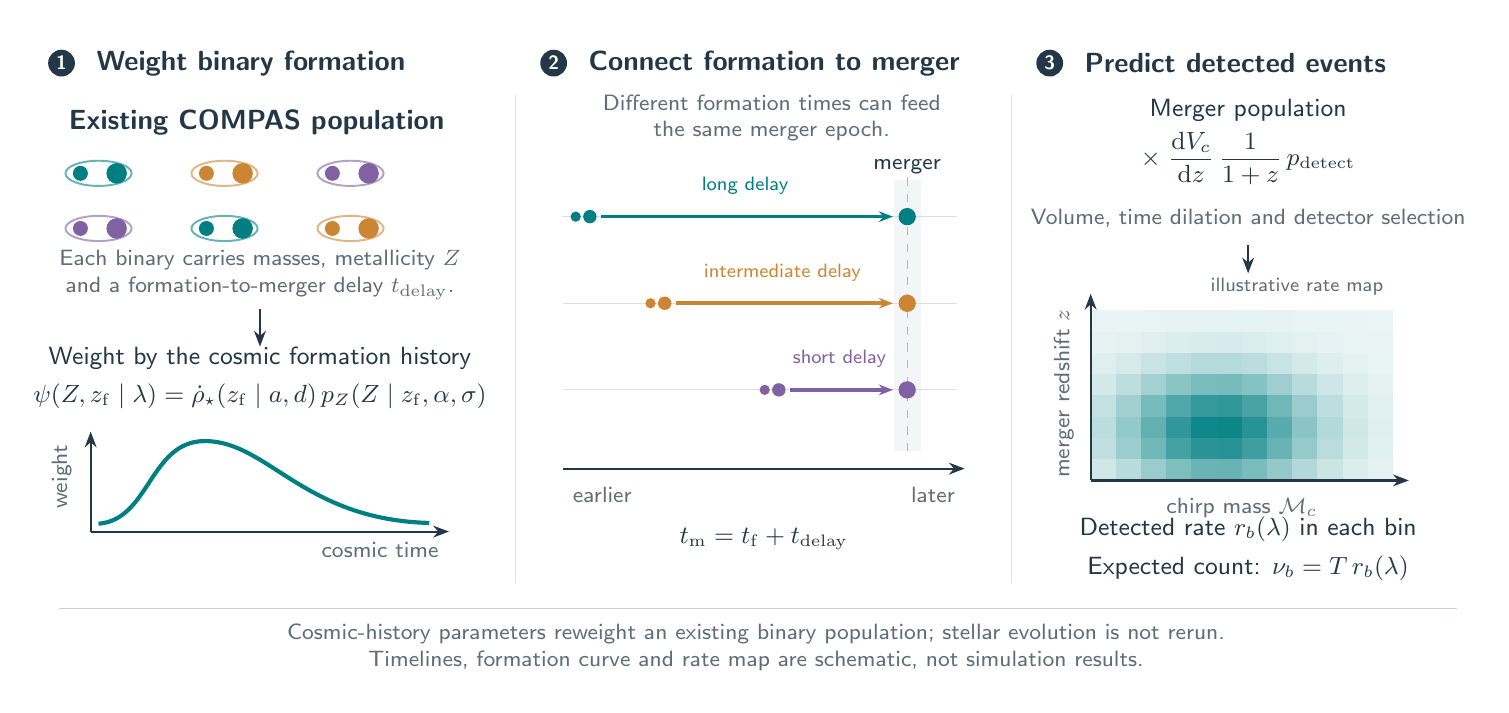
\begin{tikzpicture}[x=1cm,y=1cm,font=\sffamily\small,text=ink,
  arr/.style={-{Stealth[length=2mm]},line width=.8pt,draw=ink},
  note/.style={font=\sffamily\footnotesize,text=muted,align=center}]
\path[use as bounding box] (-.25,-1.25) rectangle (18.2,7.1);
% Three reading regions, with no enclosing flowchart boxes.
\foreach \x/\n/\heading in {0/1/Weight binary formation,6.25/2/Connect formation to merger,12.55/3/Predict detected events}{
  \fill[ink] (\x+.18,6.65) circle (.17);
  \node[white,font=\sffamily\scriptsize\bfseries] at (\x+.18,6.65) {\n};
  \node[anchor=west,font=\sffamily\bfseries] at (\x+.5,6.65) {\heading};
}
\draw[black!12] (5.95,.05)--(5.95,6.25);
\draw[black!12] (12.25,.05)--(12.25,6.25);

% Fixed population: symbolic pairs, with metallicity encoded by colour.
\node[anchor=west,font=\sffamily\bfseries] at (.15,5.9) {Existing COMPAS population};
\foreach \x/\y/\c in {.65/5.25/teal,2.25/5.25/gold,3.85/5.25/purple,.65/4.55/purple,2.25/4.55/teal,3.85/4.55/gold}{
  \draw[\c!60,line width=.7pt] (\x,\y) ellipse (.42 and .16);
  \fill[\c] (\x-.23,\y) circle (.095);
  \fill[\c] (\x+.23,\y) circle (.13);
}
\node[note] at (2.7,3.96) {Each binary carries masses, metallicity $Z$\\ and a formation-to-merger delay $t_{\rm delay}$.};
\draw[arr] (2.7,3.53)--(2.7,3.05);
\node[align=center] at (2.7,2.65) {Weight by the cosmic formation history\\[3pt]
  $\psi(Z,z_{\rm f}\mid\lambda)=\dot\rho_\star(z_{\rm f}\mid a,d)\,p_Z(Z\mid z_{\rm f},\alpha,\sigma)$};
% A small history curve is deliberately qualitative.
\draw[arr] (.55,.7)--(5.1,.7) node[below left,note] {cosmic time};
\draw[arr] (.55,.7)--(.55,1.97);
\node[note,rotate=90] at (.18,1.4) {weight};
\draw[teal,line width=1.5pt] (.65,.8) .. controls (1.3,.85) and (1.3,1.85) .. (2,1.85)
  .. controls (2.8,1.85) and (3.25,.85) .. (4.85,.81);

% Aligned timelines: each coloured pair forms at a different time and
% reaches the same vertical merger slice after its own delay.
\node[note] at (9.2,5.95) {Different formation times can feed\\ the same merger epoch.};
\fill[pale] (10.75,1.72) rectangle (11.1,5.17);
\draw[ink!35,dashed] (10.92,1.72)--(10.92,5.3);
\node[font=\sffamily\footnotesize,anchor=south] at (10.92,5.12) {merger};
\foreach \xf/\yy/\cc/\lab in {6.8/4.7/teal/long delay,7.75/3.6/gold/intermediate delay,9.2/2.5/purple/short delay}{
  \draw[black!13] (6.55,\yy)--(11.55,\yy);
  \fill[\cc] (\xf-.09,\yy) circle (.065);
  \fill[\cc] (\xf+.09,\yy) circle (.085);
  \draw[-{Stealth[length=1.8mm]},\cc,line width=1.3pt] (\xf+.23,\yy)--(10.74,\yy);
  \fill[\cc] (10.92,\yy) circle (.11);
  \node[font=\sffamily\scriptsize,text=\cc,anchor=south] at ({(\xf+10.92)/2},\yy+.16) {\lab};
}
\draw[arr] (6.55,1.5)--(11.65,1.5);
\node[note,anchor=north west] at (6.55,1.39) {earlier};
\node[note,anchor=north east] at (11.65,1.39) {later};
\node at (9.1,.61) {$t_{\rm m}=t_{\rm f}+t_{\rm delay}$};

% Selection is applied to merger rates, before constructing detected counts.
\node[align=center] at (15.25,5.65) {Merger population\\[3pt]
  $\times\;\dfrac{\mathrm dV_c}{\mathrm dz}\,\dfrac{1}{1+z}\,p_{\rm detect}$};
\node[note] at (15.25,4.68) {Volume, time dilation and detector selection};
\draw[arr] (15.25,4.34)--(15.25,3.98);
% Analytic, dimensionless toy map: no physical or fitted numbers are implied.
\begin{scope}[shift={(13.25,1.35)}]
\foreach \i in {0,...,11}{
  \foreach \j in {0,...,7}{
    \pgfmathsetmacro{\tone}{8+88*exp(-((\i-4.6)/3.7)^2-((\j-1.9)/2.6)^2)}
    \fill[teal!\tone!white] (\i*.32,\j*.27) rectangle +( .322,.272);
  }
}
\draw[arr] (0,0)--(4.04,0);
\draw[arr] (0,0)--(0,2.37);
\node[note] at (1.92,-.35) {chirp mass $\mathcal M_c$};
\node[note,rotate=90] at (-.34,1.1) {merger redshift $z$};
\node[note,anchor=south east,font=\sffamily\scriptsize] at (3.84,2.23) {illustrative rate map};
\end{scope}
\node[align=center] at (15.25,.48) {Detected rate $r_b(\lambda)$ in each bin\\[3pt]
  Expected count: $\nu_b=T\,r_b(\lambda)$};

\draw[ink!25] (.15,-.28)--(17.9,-.28);
\node[note,text width=17cm] at (9,-.77) {Cosmic-history parameters reweight an existing binary population; stellar evolution is not rerun.\\
Timelines, formation curve and rate map are schematic, not simulation results.};
\end{tikzpicture}
\end{document}
